\documentclass[12pt,a4paper]{article}
\usepackage[a4paper,top=1.5cm, bottom=1.5cm, left=1.5cm, right=1.5cm]{geometry}
\usepackage[T2A]{fontenc}
\usepackage[utf8]{inputenc}
\usepackage[russian]{babel}
\usepackage{amsmath}
\usepackage{amssymb}
\usepackage{graphicx}
\usepackage{floatrow}
\usepackage{booktabs}
\usepackage{wrapfig}
\usepackage{lipsum}
\usepackage{subcaption}
\usepackage{indentfirst}

\newcommand{\figref}[1]{(См. рис. \ref{#1})}
\newcommand{\e}[1]{\text{$\cdot10^{#1}$}}

\title{Лабораторная работа 2.2.1\\ Исследование взаимной диффузии газов}
\author{Симанкович Александр \\ Б01-104}
\date{06.04.2022}

\usepackage{float}
\restylefloat{table}

\begin{document}
	\maketitle
	
	\section*{Цель работы}
	Регистрация зависимости концентрации гелия в воздухе от времени с помощью датчиков теплопроводности при разных начальных давлениях смеси газов
	
	Определение коэффициента диффузии по результатам измерений.
	
	\section*{Оборудование и приборы} 
	Измерительная установка; форвакуумный насос; баллон с газом (гелий); манометр; источник питания;
	магазин сопротивлений; гальванометр; секундомер.
	
	\subsection*{Теоретическое введение}
	Диффузией называют самопроизвольное взаимное проникновение веществ друг в друга, происходящее вследствие хаотичного теплового движения молекул.
	При перемешивании молекул разного сорта говорят о взаимной (или концентрационной) диффузии.
	Диффузия в системе, состоящей из двух компонентов $a$ и $b$ (бинарная смесь), подчиняется закону Фика: плотности потока компонентов $j_{a, b}$ (количество частиц, пересекающих единичную площадку в единицу времени) пропорциональны градиентам их концентраций $\nabla n_{a, b}$, что в одномерном случае можно записать как
	\begin{equation}
		j_a = -D \dfrac{\partial n_a}{\partial x},~j_b = -D \dfrac{\partial n_b}{\partial x},
	\end{equation}
	где $D$ -- коэффициент взаимной диффузии компонентов. Знак «минус» отражает тот факт, что диффузия идёт в направлении выравнивания концентраций.
	Равновесие достигается при равномерном распределении вещества по объёму сосуда ($\dfrac{\partial n}{\partial x} = 0$).

	В данной работе исследуется взаимная диффузия гелия и воздуха. Давление $P$ и температура $T$ в условиях опыта предполагаются неизменными.

	Приведём теоретическую оценку для коэффициента диффузии.
	В работе концентрация гелия, как правило, мала ($n_{He} \ll n_{\text{в}}$).
	Кроме того, атомы гелия существенно легче молекул, составляющих воздух ($\mu_{He} \ll \mu_{N_2}, \mu_{O_2}$), значит и их средняя тепловая скорость велика по сравнению с остальными частицами.
	Поэтому перемешивание газов в работе можно приближенно описывать как диффузию примеси лёгких частиц $He$ на практически стационарном фоне воздуха.
	Коэффициент диффузии в таком приближении равен 
	\begin{equation}\label{eq:lambda}
		D = \dfrac{1}{3} \lambda \overline{v},
	\end{equation}
	где $\overline{v} = \sqrt{\dfrac{8RT}{\pi \mu}}$ -- средняя тепловая скорость частиц примеси, $\lambda = \dfrac{1}{n_0 \sigma}$ -- их длина свободного пробега, $n_0$ -- концентрация рассеивающих центров (фона), $\sigma$ -- сечение столкновения частиц примеси с частицами фона.

	Таким образом, теория предсказывает, что коэффициент диффузии бинарной смеси обратно пропорционален давлению в системе $D \propto \dfrac{1}{P}$, и не зависит от пропорций компонентов.

\section*{Экспериментальная установка}
	Для исследования взаимной диффузии газов и измерения коэффициента взаимной диффузии $D$ используется два сосуда объёмами $V_1$ и $V_2$ ($V_1 \approx V_2 \equiv V$), соединенные трубкой длины $L$ и сечения $S$ (рис. 1) (Параметры установки внесены в таблицу \ref{tab:scheme}).
	Предполагается, что сосуды заполнены смесью двух газов при одинаковом давлении, но с различной концентрацией компонентов.
	Вследствие взаимной диффузии, проходящей в соединительной трубке, концентрации компонентов в сосудах с течением времени выравниваются.

	\begin{figure}[h]
		\centering
		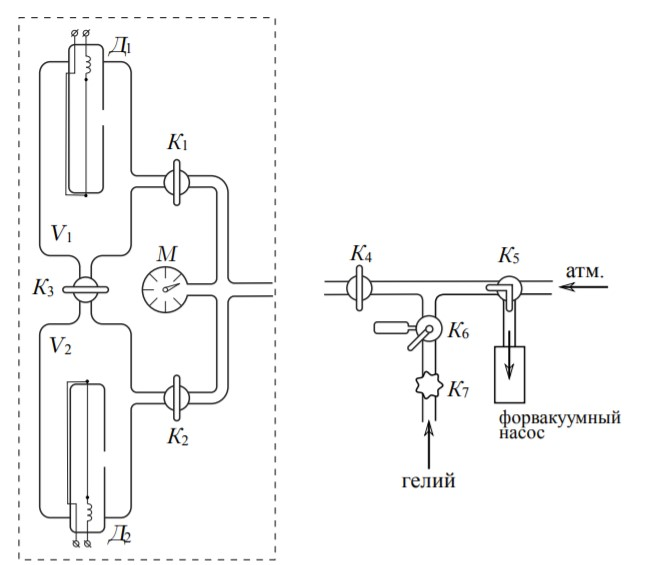
\includegraphics[width=0.8\linewidth]{res/scheme}
		\caption{Схема установки}
		\label{fig:scheme}
	\end{figure}
	
	\begin{equation}
		\dfrac{d(\Delta n)}{dt} = - \dfrac{\Delta n}{\tau},
	\end{equation}
	где введено обозначение
	\begin{equation}
		\tau = \dfrac{1}{D} \dfrac{VL}{2S}.
	\end{equation}
	Интегрируя $(6)$, получаем, что разность концентраций будет убывать по экспоненциальному закону
	\begin{equation}
		\Delta n = \Delta n_0 e^{-t/\tau},
	\end{equation}
	где $\Delta n_0$ --— разность концентраций примеси в сосудах в начальный момент времени.
	Видно, что величина $\tau$ есть характерное время выравнивания концентраций между сосудами.
	Оно определяется геометрическими размерами установки и коэффициентом диффузии.
	
	Для измерения сопротивлений используется мостовая схема, позволяющая определять разность показаний датчиков с высокой точностью.
	Мост балансируется при заполнении сосудов (и датчиков) одной и той же смесью.
	При заполнении сосудов смесями различного состава возникает «разбаланc» моста.
	При незначительном различии в составах смесей показания вольтметра, подсоединённого к диагонали моста, будут пропорциональны разности концентраций примеси: $U \propto \Delta \kappa \propto \Delta n$.
	В процессе диффузии разность концентраций убывает по закону $(8)$, и значит по тому же закону изменяется напряжение: 
	\begin{equation}
		U = U_0 e^{-t/\tau},
	\end{equation}
	где $U_0$ --- показание гальванометра в начальный момент времени.
	Измеряя экспериментально зависимость $U(t)$, можно получить характерное время процесса $\tau$, откуда по формуле $(8)$ определить коэффициент диффузии $D$.


	\begin{table}[h]
		\centering
		\caption{Параметры установки}
		\label{tab:scheme}
		\footnotesize
		\begin{tabular}{ll}
			
			\toprule
			Параметр установки & Значение \\
			\midrule
			V & $(420\pm10) $ $\text{см}^3$ \\
			$L/S$ & $(9.0\pm1.0)$ $ \text{см}^{-1}$ \\
			$P_{\text{гел.}}$ & $0.2 P_{\text{раб}}$ \\
			$P_{\text{возд.}}$ & $1.7 P_{\text{раб}}$ \\
			\bottomrule
			
		\end{tabular}
		
	\end{table} 

\section*{Ход работы}
	
	Для смеси гелий-воздух исследуем зависимость коэффициента взаимной диффузии о начального давления в системе. Для этого будем фиксировать с помощью компьютера в лаборатории зависимость показаний вольтметра от времени, прошедшего с начала эксперимента. Полученные результаты наглядно представлены в виде графиков зависимости $U(t)$ на рисунке \ref{fig:ut}.
	
	Для нахождения коэффициентов взаимной диффузии линеаризируем зависимость $U(t)$. Для наглядной оценки качества линеаризации приведены графики зависимостей $\ln{U}(t)$ на рисунке \ref{fig:lnut}. Статистическая обработка была проведена \textbf{методом наименьших квадратов}. Обосновать выбор метода это можно тем, что погрешность отдельного измерения относительна мала, а количество точек, снятых с помощью компьютера велико ($\approx400$ точек на серию). Вся статистическая обработка занесена в таблицу \ref{tab:dstat}.
	
	Расчет коэффициентов взаимной диффузии проведем с помощью следующих формул:
	
	$$D = a \dfrac{VL}{2S},$$ 
	$$\sigma_D = D \sqrt{\varepsilon_{a}^2 + \varepsilon_{V}^2 +  \varepsilon_{L/S}^2},$$
	где $\varepsilon_{x} = \frac{\sigma_x}{x}$ - соответствующие относительные погрешности случайных величин,
	$a$ - коэффициент наклона линейной зависимости.
	
	
	\begin{table}[H]
		\centering
		\caption{Статистическая обработка зависимости $\ln{U}(t)$}
		\label{tab:dstat}
		\footnotesize
		\begin{tabular}{lllllr}
			\toprule
			$P_{\text{раб}}$, торр & $a$ & $\sigma_a$ & $b$ & $\sigma_b$ & $D\pm\sigma_D$, $\frac{\text{см}^2}{\text{c}}$\\
			\midrule
			44.5  &  -0.003855 & 5\e{-6}  &  3.15 & 0.05 & $7.29\pm 0.19$ \\
			81.7  &  -0.002427 & 1.0\e{-6}  &  3.03 & 0.03 & $4.59\pm 0.12$ \\
			133.7  &  -0.0015507 & 8\e{-7}  &  3.03 & 0.07 & $2.93\pm 0.08$ \\
			170.9  &  -0.001244 & 1.3\e{-6}  &  3.00 & 0.14 & $2.35\pm 0.06$ \\
			208.2  &  -0.001017 & 5\e{-6}  &  2.95 & 0.10 & $1.92\pm 0.05$ \\
			\bottomrule
		\end{tabular}
	\end{table}
	
	
	
	\begin{figure}[H]
		\centering
		\includegraphics[width=1\linewidth]{res/U_T}
		\caption{Зависимость $U(t)$}
		\label{fig:ut}
	\end{figure}
	
	\begin{figure}[H]
		\centering
		\includegraphics[width=1\linewidth]{res/lnU_T}
		\caption{График зависимости $\ln{U}(t)$}
		\label{fig:lnut}
	\end{figure}
	
	
	Для нахождения $D_\text{атм}$, следует экстраполировать зависимость $D(\frac{1}{P})$ к точке $\frac{1}{P_\text{атм}}$. Для этого построим график $D(\frac{1}{P})$ (см. рис. \ref{fig:d1p}), чтобы убедиться в целесообразности экстраполяции. Затем с помощью метода наименьших квадратов проведем расчет коэффициентов линейной зависимости. Статистическую обработку занесем в таблицу \ref{tab:d1p}.
	
	Погрешность $D_\text{атм}$ оценим с помощью закона накопления ошибок:
	$$\sigma_{D_\text{атм}} = \sqrt{\sigma_b^2 + \left(\frac{1}{P_\text{атм}}\sigma_a\right)^2}$$
	
	
	
	
	\begin{figure}[H]
		\centering
		\includegraphics[width=1\linewidth]{res/D_1P}
		\caption{График зависимости $D(\frac{1}{P})$}
		\label{fig:d1p}
	\end{figure}
	
	\begin{table}[H]
		\centering
		\caption{Статистическая обработка зависимости $D(\frac{1}{P})$}
		\label{tab:d1p}
		\footnotesize
		\begin{tabular}{lcccccc}
			\toprule
			Зависимость & $a$ & $\sigma_a$ & $b$ & $\sigma_b$ & $\frac{1}{P_\text{атм}}$, торр$^{-1}$ & $D_\text{атм}\pm\sigma_D$, $\frac{\text{см}^2}{\text{c}}$\\
			\midrule
			$D = a\frac{1}{P} + b$  &  355 & 12 &  0.2519 & 0.0007 & 0.001318 & $0.72\pm 0.02$ \\
			\bottomrule
		\end{tabular}
	\end{table}
	\clearpage
	Найдем длину свободного пробега с помощью формулы \ref{eq:lambda}:
	$$\lambda_{\text{атм}} = 3 D_\text{атм} \sqrt{\frac{\pi \mu}{8RT}} = (172 \pm 4) \text{ нм}$$
	$$\sigma_{\lambda_{\text{атм}}} = \lambda_{\text{атм}} \varepsilon_{D_\text{атм}}$$
	
	Аналогично для $\sigma_{\text{He-возд.}}$ получаем:
	$$\sigma_{\text{He-возд.}} = \frac{1}{n_0\lambda} = \frac{kT}{P_\text{атм}\lambda_{\text{атм}}} \approx (3.15 \pm 0.07)\e{-19} \text{ м}^2$$
	$$ \sigma_{\sigma_{\text{He-возд.}}} = \sigma_{\sigma_{\text{He-возд.}}}\varepsilon_{\lambda_{\text{атм}}}$$

\section*{Вывод}
	При обработке эксперимента получены вполне достоверные результаты.
	Стоит отметить, что основную погрешность в определении величин внесла систематическая ошибка параметров установки, а также систематическая погрешность, которая тяжело поддается какой-либо оценке. Это следует из того, что относительные погрешности коэффициентов взаимной диффузии $D$ практически не зависят от случайной ошибки определения параметров линейной зависимости $\ln{U}(t)$, в чем можно убедиться, глядя нa таблицу \ref{tab:dstat}. 
	Получено значение коэффициента взаимной диффузии при атмосферном давлении:
	$$D_\text{атм} = (0.72\pm 0.02)\frac{\text{см}^2}{\text{c}}, \left( D_\text{таб.} = 0.62 \frac{\text{см}^2}{\text{c}}, \text{ при } t = 0^{\circ} C\right).$$
	
	Также определена длина свободного пробега атомов He и эффективная площадь сечения:
	$$\lambda_{\text{атм}} = (172 \pm 4) \text{ нм}$$
	
	$$\sigma_{\text{He-возд.}} = (3.15 \pm 0.07)\e{-19} \text{ м}^2$$

\end{document}